%\usepackage{tikz}
%\usepackage[american]{circuitikz}
\graphicspath{{./Chapters/CH2/Pictures/}}
\let\cleardoublepage\clearpage
\section{Active Front End Rectifier Modeling}
The Grid under the study in this subsection is assumed to be a balanced three-phase grid with sinusoidal grid voltages shifted with 120 degrees between each phase. The three phase grid is star connected to three inductors which are known as boost inductors referred to $L$. Symbols are summarized in Table~\ref{tab:spmsm-notation-narrative}; equation references are provided instead of inline formulas to keep the text readable.

\begin{figure}[htbp]
    \centering
    % If the diagram is too wide for your margins, uncomment the \resizebox line below 
    % and the matching closing brace at the end of the circuitikz environment.
    \resizebox{\textwidth}{!}{%
    \begin{circuitikz}[american, thick]
        % --- Define Grid Coordinates ---
        % Y-coordinates for vertical alignment
        \def\yTop{7}       % Top DC Bus
        \def\yBot{0}       % Bottom DC Bus
        \def\yA{5}         % Phase A horizontal line
        \def\yB{3.5}       % Phase B horizontal line
        \def\yC{2}         % Phase C horizontal line
        \def\ySwTop{6}     % Centered y-coord for upper switches
        \def\ySwBot{1}     % Centered y-coord for lower switches
    
        % X-coordinates for horizontal spacing
        \def\xNeu{0}       % Common neutral wire
        \def\xSrc{1}       % AC Sources
        \def\xR{2.5}       % Resistors (Rs)
        \def\xL{4.5}       % Inductors (Ls)
        \def\xEndL{6.5}    % End of inductor line
        \def\xLegA{8}      % Rectifier Leg 1
        \def\xLegB{10.5}   % Rectifier Leg 2
        \def\xLegC{13}     % Rectifier Leg 3
        \def\xCap{15.5}    % DC Capacitor
        \def\xLoad{18}     % Resistive Load
    
        % ==========================================
        % 1. LINE SIDE (AC SOURCES & IMPEDANCES)
        % ==========================================
        
        % Common neutral wire on the far left
        \draw (\xNeu,\yA) -- (\xNeu,\yC);
    
        % Phase A 
        \draw (\xNeu,\yA) -- (\xSrc,\yA)
              to[sV, l=$V_a$] (\xR,\yA)
              to[R, l=$R_s$] (\xL,\yA)
              to[L, l=$L_s$] (\xEndL,\yA)
              -- (\xLegA,\yA) node[circ]{}; % Intersection dot at Leg 1
    
        % Phase B 
        \draw (\xNeu,\yB) -- (\xSrc,\yB)
              to[sV, l=$V_b$] (\xR,\yB)
              to[R, l=$R_s$] (\xL,\yB)
              to[L, l=$L_s$] (\xEndL,\yB)
              -- (\xLegB,\yB) node[circ]{}; % Intersection dot at Leg 2
    
        % Phase C 
        \draw (\xNeu,\yC) -- (\xSrc,\yC)
              to[sV, l=$V_c$] (\xR,\yC)
              to[R, l=$R_s$] (\xL,\yC)
              to[L, l=$L_s$] (\xEndL,\yC)
              -- (\xLegC,\yC) node[circ]{}; % Intersection dot at Leg 3
    
        % Current flow arrows (i_a, i_b, i_c)
        \draw[-latex, line width=1.2pt] (\xEndL+0.3, \yA+0.3) -- (\xEndL+1.3, \yA+0.3) node[midway, above] {$i_a$};
        \draw[-latex, line width=1.2pt] (\xEndL+0.3, \yB+0.3) -- (\xEndL+1.3, \yB+0.3) node[midway, above] {$i_b$};
        \draw[-latex, line width=1.2pt] (\xEndL+0.3, \yC+0.3) -- (\xEndL+1.3, \yC+0.3) node[midway, above] {$i_c$};
    
        % ==========================================
        % 2. RECTIFIER BRIDGE (ACTIVE SWITCHES)
        % ==========================================
        
        % Top and Bottom DC buses
        \draw (\xLegA,\yTop) -- (\xLoad,\yTop);
        \draw (\xLegA,\yBot) -- (\xLoad,\yBot);
    
        % Instantiate IGBTs with body diodes as perfectly aligned nodes
        % Upper Switches
        \node[nigbt, bodydiode] (S1) at (\xLegA, \ySwTop) {};
        \node[nigbt, bodydiode] (S2) at (\xLegB, \ySwTop) {};
        \node[nigbt, bodydiode] (S3) at (\xLegC, \ySwTop) {};
    
        % Lower Switches
        \node[nigbt, bodydiode] (S1b) at (\xLegA, \ySwBot) {};
        \node[nigbt, bodydiode] (S2b) at (\xLegB, \ySwBot) {};
        \node[nigbt, bodydiode] (S3b) at (\xLegC, \ySwBot) {};
    
        % Wire up Leg 1
        \draw (S1.C) -- (\xLegA, \yTop);
        \draw (S1.E) -- (S1b.C);
        \draw (S1b.E) -- (\xLegA, \yBot);
    
        % Wire up Leg 2
        \draw (S2.C) -- (\xLegB, \yTop);
        \draw (S2.E) -- (S2b.C);
        \draw (S2b.E) -- (\xLegB, \yBot);
    
        % Wire up Leg 3
        \draw (S3.C) -- (\xLegC, \yTop);
        \draw (S3.E) -- (S3b.C);
        \draw (S3b.E) -- (\xLegC, \yBot);
    
        % Add precise bold switch labels to the right of the components
        \node at (\xLegA+0.8, \ySwTop) {$\mathbf{S_1}$};
        \node at (\xLegB+0.8, \ySwTop) {$\mathbf{S_3}$};
        \node at (\xLegC+0.8, \ySwTop) {$\mathbf{S_5}$};
    
        \node at (\xLegA+0.8, \ySwBot) {$\mathbf{S_4}$};
        \node at (\xLegB+0.8, \ySwBot) {$\mathbf{S_6}$};
        \node at (\xLegC+0.8, \ySwBot) {$\mathbf{S_2}$};
    
        % ==========================================
        % 3. LOAD SIDE (DC LINK & RESISTOR)
        % ==========================================
        
        % DC Link Capacitor
        \draw (\xCap,\yTop) to[C, l_=$C$] (\xCap,\yBot);
    
        % Standard Resistor Load (Label moved to the left using l_)
        \draw (\xLoad, \yTop) to[R, l_=$R_{load}$] (\xLoad, \yBot);
    
        % Add + and - polarities on the right side of the load resistance
        \node[font=\Large] at (\xLoad+0.4, \yTop-0.8) {$+$};
        \node[font=\Large] at (\xLoad+0.4, \yBot+0.8) {$-$};
    
        % V_dc Voltage Arrow (Moved to the right of the resistor)
        \draw[-latex, line width=1.2pt] (\xLoad+1.2, \yBot+1.5) -- (\xLoad+1.2, \yTop-1.5) node[midway, right] {$V_{dc}$};
    
    \end{circuitikz}
     } % Uncomment this brace if you uncommented the \resizebox command above
    
    \caption{Three-phase Active front-end rectifier.}
    \label{fig:afe_schematic}
\end{figure}



%\begin{figure}[h]
%	\centering
%		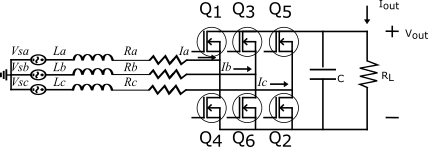
\includegraphics[width=\textwidth]{AFE_Final_Gates}
%	\caption{Active Front End Rectifier}
%	\label{fig:AFE_Modeling}
%\end{figure}
The grid voltage of each phase is described by a using KVL voltage equations that includes resistive drop of each boost inductor and the rate of change of flux linkage. This relationship is written in Equation~\eqref{eq:narr-abc-phase} for a generic phase and in Equation~\eqref{eq:narr-abc-vector} in vector form for all three phases. The resistive term represents the losses of the resistance of the boost inductor, while the derivative of flux linkage represents the boost inductor and its core losses.

\begin{table}[H]
\centering
\caption{Symbols used in the SPMSM model}
\label{tab:spmsm-notation-narrative}
\begin{tabular}{ll}
\hline
Symbol & Description \\
\hline
$R$ & Boost inductor resistance \\
$L$ &   Boost inductor inductance \\
$C$ &   DC Link Capacitor \\
$R_l$ & Load resistance \\
$v_a, v_b, v_c$ & Three phase grid voltages \\
$v_{conva}, v_{convb}, v_{convc}$ & Three phase converter voltages \\
$i_a, i_b, i_c$ & Three phase grid currents \\
$v_\alpha, v_\beta$ & Stationary-frame grid voltages \\
$v_{conv\alpha}, v_{conv\beta}$ & Stationary-frame converter voltages \\
$i_\alpha, i_\beta$ & Stationary-frame grid currents \\
$v_{sd}, v_{sq}$ & Synchronous dq frame grid voltages \\
$i_d, i_q$ & Synchronous dq frame currents \\
$v_{convd}, v_{convq}$ & Synchronous dq frame converter voltages \\
$v_{dc}$ & Output DC Link voltages \\
$s_d, s_q$ & Synchronous dq frame switching function \\
$\theta$ & Electrical angle \\
$\omega$ & Electrical frequency \\
$P$ & Three phase active power of the grid \\
$Q$ & Three phase reactive power of the grid \\

\hline
\end{tabular}
\end{table}

\begin{equation}
\label{eq:narr-abc-phase}
v_\ell - v_{conv\ell} = R\, i_\ell + L\frac{\mathrm di_\ell}{\mathrm d t} \,, \qquad \ell \in \{a,b,c\} .
\end{equation}

\begin{equation}
\label{eq:narr-abc-vector}
\begin{bmatrix} v_a \\ v_b \\ v_c \end{bmatrix} - 
\begin{bmatrix} v_{conva} \\ v_{convb} \\ v_{convc} \end{bmatrix}
= R \begin{bmatrix} i_a \\ i_b \\ i_c \end{bmatrix}
+ L\frac{\mathrm d}{\mathrm d t} \begin{bmatrix} i_a \\ i_b \\ i_c \end{bmatrix} .
\end{equation}

For active front end rectifier, the phase flux linkages consist of a  term proportional to phase current and an inductive term that depends on the inductance of the boost rectifier. Equations~\eqref{eq:narr-abc-phase}–\eqref{eq:narr-abc-vector} define the relationship between the three phase grid voltages and the three phase converter voltages by using KVL equations.

Applying the power‑invariant Clarke transform to Equations~\eqref{eq:narr-abc-phase}–\eqref{eq:narr-abc-vector} yields the stationary‑frame voltages in Equations~\eqref{eq:add-ab-volt-a} and \eqref{eq:add-ab-volt-b}. The resistive and inductive parts preserve their form under the linear transform. 

\begin{equation}
\label{eq:narr-clarke}
\begin{bmatrix} v_\alpha \\ v_\beta \end{bmatrix}
= \tfrac{2}{3}
\begin{bmatrix}
1 & -\tfrac{1}{2} & -\tfrac{1}{2} \\
0 & \tfrac{\sqrt 3}{2} & -\tfrac{\sqrt 3}{2}
\end{bmatrix}
\begin{bmatrix} v_a \\ v_b \\ v_c \end{bmatrix} .
\end{equation}

\begin{equation}
\label{eq:add-ab-volt-a}
 v_\alpha = R \, i_\alpha + L \, \frac{\mathrm d i_\alpha}{\mathrm d t} + v_{conv\alpha} .
\end{equation}
\begin{equation}
\label{eq:add-ab-volt-b}
 v_\beta = R \, i_\beta + L \, \frac{\mathrm d i_\beta}{\mathrm d t} + v_{conv\beta} .
\end{equation}

The Park transform rotates the stationary axes so that one axis is aligned with phase A. In this frame, steady operating points correspond to nearly constant quantities, which simplifies control and analysis. The mappings for current and voltage are given in Equations~\eqref{eq:narr-park-i} to \eqref{eq:narr-park-v}.

\begin{equation}
\label{eq:narr-park-i}
\begin{bmatrix} i_d \\ i_q \end{bmatrix}
= \begin{bmatrix} \cos \theta & \sin \theta \\ -\sin \theta & \cos \theta \end{bmatrix}
\begin{bmatrix} i_\alpha \\ i_\beta \end{bmatrix} .
\end{equation}

\begin{equation}
\label{eq:narr-park-v}
\begin{bmatrix} v_d \\ v_q \end{bmatrix}
= \begin{bmatrix} \cos \theta & \sin \theta \\ -\sin \theta & \cos \theta \end{bmatrix}
\begin{bmatrix} v_\alpha \\ v_\beta \end{bmatrix} .
\end{equation}

In the rotating frame, The direct- and quadrature-axis voltage balances are listed in Equations~\eqref{eq:narr-dq-vd} and \eqref{eq:narr-dq-vq}. The electrical angular frequency terms couple the axes and motivate decoupling in controllers.

\begin{equation}
\label{eq:narr-dq-vd}
v_{sd} = R\, i_d + \frac{\mathrm d i_d}{\mathrm d t} - \omega L i_q + v_{convd}.
\end{equation}

\begin{equation}
\label{eq:narr-dq-vq}
v_{sq} = R\, i_q + \frac{\mathrm d i_q}{\mathrm d t} + \omega L i_d + v_{convq}.
\end{equation}

Substituting the grid current derivative relations into the voltage balances leads to first-order dynamics for the axis currents. Equation~\eqref{eq:narr-dq-did} shows that the direct-axis current is driven by the direct-axis voltage, opposed by resistive drop, and coupled to the quadrature current through electrical frequency-dependent term. Equation~\eqref{eq:narr-dq-diq} shows that the quadrature-axis current is driven by the quadrature-axis voltage, opposed by resistive drop, and coupled to the quadrature current through electrical frequency-dependent term. These forms motivate feedforward decoupling in advanced controllers.

\begin{equation}
\label{eq:narr-dq-did}
\dot{i}_d = \frac{1}{L} \Big( v_{sd} - R i_d + \omega L i_q - v_{convd}\Big) .
\end{equation}

\begin{equation}
\label{eq:narr-dq-diq}
\dot{i}_q = \frac{1}{L} \Big( v_{sq} - R i_q - \omega L i_d - v_{convq}\Big) .
\end{equation}

The instantaneous three-phase electrical active power expressed in synchronous coordinates is a weighted inner product of voltage and current components, shown in Equation~\eqref{eq:narr-pe}. While The instantaneous three-phase electrical reactive power expressed in synchronous coordinates is a weighted inner product of voltage and current components, shown in Equation~\eqref{eq:narr-qe}.
\begin{equation}
\label{eq:narr-pe}
P = \tfrac{3}{2} \big( v_{sd} i_d + v_{sq} i_q \big) .
\end{equation}

\begin{equation}
\label{eq:narr-qe}
Q = \tfrac{3}{2} \big( v_{sq} i_d - v_{sd} i_q \big) .
\end{equation}


The above equations represent the instantaneous input active and reactive power supplied by the grid. Equation~\eqref{eq:narr-dclink} states the relation between the output DC link voltage and the output power drawn by the load. Those equations are necessary for the derivation of the transfer functions of the grid currents in the dq synchronous frame and the transfer function of the DC link voltage which are crucial for simulation and control design.

\begin{equation}
\label{eq:narr-dclink}
C\,\dot v_{dc} = \tfrac{3}{2} \big( S_d i_d + S_q i_q \big) - \frac{v_{dc}}{R_l} .
\end{equation}




% ==========================================================
% Subsection: Ideal Two-Level Inverter — Average (PWM) Model
% Requires: \usepackage{amsmath}
% ==========================================================

% ==========================================================
% Subsection: Ideal Two-Level Inverter — Average Model with SVM Duty Cycles
% Requires: \usepackage{amsmath}
% ==========================================================

% ==========================================================
% Subsection: Ideal Two-Level Inverter — Average Model Driven by SVM Duty Cycles
% Requires: \usepackage{amsmath}
% ==========================================================

\section{System Characterestics}
\label{subsec:motor-params-3col}

% In your preamble:
% \usepackage{booktabs}

% In your preamble:
% \usepackage{booktabs}

% Preamble: \usepackage{booktabs}
This subsection summarizes the parameters used throughout the modeling, control, and experiments as shown in  Table~\ref{tab:drive-motor-params};
\begin{table}[H]
	\centering
	\caption{Load and Active Front-End Rectifier parameters used in the experiments.}
	\label{tab:drive-motor-params}
	\begin{tabular}{l c r}
		\toprule
		\textbf{Parameter} & \textbf{Symbol} & \textbf{Value} \\
		\midrule
		DC Bus Voltage (V)                    & $V_{\mathrm{dc}}$    &600\\
		Switching Frequency (kHz)             & $f$                  &10  \\
		Dead Time ($\mu$s)                    & $T_{\mathrm{dead}}$  &2.5  \\
		Turn-on Time ($\mu$s)                 & $T_{\mathrm{ON}}$    &0.3  \\
		Turn-off Time ($\mu$s)                & $T_{\mathrm{OFF}}$   &0.3  \\
		Switch Threshold Voltage (V)          & $V_{\mathrm{ce0}}$   &0.4  \\
		Switch Turn-on Resistance ($\Omega$)  & $R_{\mathrm{ce}}$    &0.7  \\
		Diode Threshold Voltage (V)           & $V_{d0}$             &0.4  \\
		Diode Turn-on Resistance ($\Omega$)   & $R_d$                &0.7  \\
		\addlinespace[2pt]
		Inductor Resistance ($\Omega$)          & $R$                &0.55  \\
		Boost Inductor Inductance (H)               & $L$                &0.0185  \\
		Rated Supply Current per phase (A)                     & $I_{\mathrm{max}}$ &10 \\
		Rated Output Power (W)                   & $Pout_{\mathrm{rated}}$ &1200  \\
		Rated Load Current (A)                   & $I_{\mathrm{dcrated}}$ &2  \\
		\bottomrule
	\end{tabular}
\end{table}

\section{Vector Oriented Control (VOC)}
The foundation of the VOC strategy relies on the accurate synchronization with the AC grid, typically achieved through a Phase-Locked Loop (PLL). The PLL continuously extracts the grid voltage phase angle, establishing a reliable synchronization signal that allows the control system to align its rotating reference frame directly with the grid voltage vector. This precise alignment facilitates the core mechanism of VOC: the application of mathematical coordinate transformations to simplify time-varying, coupled three-phase signals. Specifically, the stationary three-phase grid variables—voltages and currents in the $abc$ frame—are first reduced to a two-phase orthogonal stationary frame (the $\alpha\beta$ frame) via the Clarke transformation. Subsequently, the Park transformation utilizes the PLL-derived phase angle to project these $\alpha\beta$ variables onto a synchronously rotating $dq$-axis reference frame.Within this synchronously rotating domain, the fundamental alternating grid variables appear as DC quantities in steady-state, which significantly simplifies the design and tuning of the linear controllers. Crucially, by aligning the $d$-axis perfectly with the grid voltage vector, the $q$-axis voltage component is inherently driven to zero. This mathematical alignment enables the complete decoupling of active and reactive power currents. Consequently, the $d$-axis current component ($i_d$) becomes directly proportional to the active power transferred, thereby dictating the DC-link voltage dynamics. Conversely, the $q$-axis current component ($i_q$) governs the reactive power exchange with the grid. By constraining the $q$-axis current reference to zero, the control system inherently achieves unity power factor operation.

Vector oriented control applies Clarke and Park transformations to convert the measured three-phase currents from the stationary \(abc\) frame into the synchronous \(dq\) frame for Grid Synchronisation. In that rotating frame, the grid currents appear as nearly dc quantities, which allows the grid current components in \(dq\) frame to be regulated independently using simple PI controllers. For the Active Front End Rectifier (AFE) considered here, the quadrature-axis current reference is typically set to \(i_q^{\ast}=0\) to eliminate the reactive power drawn from the grid, while the direct-axis current reference \(i_d^{\ast}\) is generated by the outer dc-link PI controller from the dc-link feedback measured. The inner \(d\)- and \(q\)-axis PI current controllers then generate the commanded voltages \(v_d^{\ast}\) and \(v_q^{\ast}\), which are transformed back to the stationary frame and synthesized by the rectifier using SVPWM. In VOC operation, the estimated electrical angle and electrical frequency supplied by the PLL are therefore essential because they define the transformation angle and preserve the decoupled current control structure. The system is shown in Figure \ref{fig:FocDiagram}.

\begin{figure}[h]
	\centering
	\resizebox{\textwidth}{!}{\begin{tikzpicture}[
    x=1cm,
    y=1cm,
    font=\small,
    >=Stealth,
    line cap=round,
    line join=round,
    signal/.style={->, line width=0.95pt},
    bus/.style={->, line width=1.05pt, double distance=1.15pt},
    plain/.style={line width=0.95pt},
    block/.style={draw, thick, fill=white, minimum width=2.45cm, minimum height=1.2cm, align=center},
    tallblock/.style={draw, thick, fill=white, minimum width=1.5cm, minimum height=2.35cm, inner sep=0pt},
    bubble/.style={circle, draw, thick, fill=white, minimum size=0.72cm, inner sep=0pt}
]

\definecolor{sensorpurple}{RGB}{233,222,236}
\definecolor{sensorblue}{RGB}{215,232,241}
\definecolor{svstroke}{RGB}{87,58,106}

\node[block, minimum width=2.15cm, minimum height=1.5cm] (speed) at (1.6,2.3) {Speed\\controller\\(PI)};

\node[bubble] (dqref) at (4.2,2.3) {$\mathit{dq}$};

\node[block, minimum width=2.95cm, minimum height=1.15cm] (qpi) at (6.35,3.1) {$q$-axis current\\controller (PI)};
\node[block, minimum width=2.95cm, minimum height=1.15cm] (dpi) at (6.35,1.5) {$d$-axis current\\controller (PI)};

\node[tallblock] (invpark) at (9.1,2.3) {};
\node[block, minimum width=2.4cm, minimum height=2.2cm] (svpwm) at (11.8,2.3) {};
\node[block, minimum width=1.85cm, minimum height=1.95cm] (inverter) at (14.6,2.3) {};

\node[circle, draw, thick, fill=white, minimum size=1.85cm, align=center] (pmsm) at (17.3,2.3) {PMSM};

\node[tallblock] (parkfb) at (9.1,-1.4) {};
\node[tallblock] (clarke) at (12.2,-1.4) {};
\node[bubble] (dqfb) at (5.6,-1.4) {$\mathit{dq}$};

\node[block, minimum width=2.85cm, minimum height=1.45cm] (observer) at (12.25,-3.7) {Position\\observer};

\begin{scope}[on background layer]
    \fill[sensorpurple] (4.55,4.05) rectangle (13.25,0.45);
    \fill[sensorblue] (4.15,0.25) rectangle (18.55,-4.55);
    \draw[black!25, thick] (4.55,4.05) rectangle (13.25,0.45);
    \draw[black!25, thick] (4.15,0.25) rectangle (18.55,-4.55);
\end{scope}

\draw[thick] (invpark.south west) -- (invpark.north east);
\node[anchor=north west] at ([xshift=2pt,yshift=-2pt]invpark.north west) {$\alpha\beta$};
\node[anchor=south east] at ([xshift=-2pt,yshift=2pt]invpark.south east) {$dq$};

\draw[thick] (parkfb.south west) -- (parkfb.north east);
\node[anchor=north west] at ([xshift=2pt,yshift=-2pt]parkfb.north west) {$dq$};
\node[anchor=south east] at ([xshift=-2pt,yshift=2pt]parkfb.south east) {$abc$};

\draw[thick] (clarke.south west) -- (clarke.north east);
\node[anchor=north west] at ([xshift=2pt,yshift=-2pt]clarke.north west) {$\alpha\beta$};
\node[anchor=south east] at ([xshift=-2pt,yshift=2pt]clarke.south east) {$abc$};

\begin{scope}[shift={(svpwm.center)}]
    \draw[thick, svstroke] (0,0.2) circle (0.43);
    \draw[thick, svstroke] (30:0.62)
        -- (90:0.62)
        -- (150:0.62)
        -- (210:0.62)
        -- (270:0.62)
        -- (330:0.62)
        -- cycle;
    \draw[thick, svstroke] (-0.53,-0.16) -- (0.53,0.56);
    \draw[thick, svstroke] (0.53,-0.16) -- (-0.53,0.56);
\end{scope}
\node[font=\small] at ($(svpwm.center)+(0,-0.68)$) {SVPWM};

\begin{scope}[shift={(inverter.center)}, line width=0.95pt]
    \draw (-0.55,0.68) -- (-0.55,-0.68);
    \draw (-0.90,0.00) -- (-0.55,0.00);
    \draw (-0.55,0.35) -- (0.10,0.78);
    \draw[-Stealth] (-0.55,-0.35) -- (0.10,-0.78);
    \draw (0.55,0.68) -- (0.55,-0.68);
    \draw (0.18,0.16) -- (0.88,0.16) -- (0.55,-0.25) -- cycle;
    \draw (0.18,-0.16) -- (0.88,-0.16);
\end{scope}
\node[font=\scriptsize, below=2pt of inverter] {Inverter};

\draw[thick] (pmsm.east) -- ++(0.7,0);
\draw[thick, ->] ($(pmsm.center)+(0.20,0.36)$) arc[start angle=25,end angle=-280,radius=0.50];
\node[font=\scriptsize, right] at ($(pmsm.east)+(0.8,0.35)$) {$\omega_r$};

\draw[signal] ($(speed.west)+(-1.2,0.35)$) node[left] {$\omega^{\ast}$} -- ($(speed.west)+(0,0.35)$);
\draw[signal] (speed.east) -- node[above] {$i_q^{\ast}$} (dqref.west);

\draw[signal] (dqref.east) -| ($(qpi.west)+(0,0.18)$);
\draw[signal] (dqref.east) -| ($(dpi.west)+(0,0.18)$);
\node[font=\scriptsize, anchor=west] at ($(dpi.west)+(-0.15,0.55)$) {$i_d^{\ast}=0$};

\draw[signal] (qpi.east) -| ($(invpark.west)+(0,0.35)$);
\draw[signal] (dpi.east) -| ($(invpark.west)+(0,-0.35)$);
\node[font=\scriptsize, anchor=south] at ($(qpi.east)!0.55!(invpark.west)+(0,0.18)$) {$v_q^{\ast}$};
\node[font=\scriptsize, anchor=north] at ($(dpi.east)!0.55!(invpark.west)+(0,-0.18)$) {$v_d^{\ast}$};

\coordinate (vabmid) at ($(invpark.east)!0.5!(svpwm.west)$);
\draw[signal] (invpark.east) -- node[above] {$v_{\alpha},v_{\beta}$} (svpwm.west);

\draw[signal] ($(svpwm.east)+(0,0.22)$) -- ($(inverter.west)+(0,0.22)$);
\draw[signal] ($(svpwm.east)+(0,-0.22)$) -- ($(inverter.west)+(0,-0.22)$);

\draw[bus] (inverter.east) -- (pmsm.west);

\coordinate (meastop) at ($(inverter.east)!0.60!(pmsm.west)$);
\coordinate (measbot) at ($(meastop |- clarke.east)$);

\draw[line width=1.0pt] (meastop) -- (measbot);
\draw[line width=1.0pt] ($(meastop)+(0.14,0)$) -- ($(measbot)+(0.14,0)$);
\node[font=\scriptsize, anchor=west] at ($(meastop)+(0.22,0.28)$) {$i_a,i_b,i_c$};

\draw[bus] (measbot) -- (clarke.east);
\draw[bus] (clarke.west) -- node[above] {$i_{\alpha},i_{\beta}$} (parkfb.east);
\draw[bus] (parkfb.west) -- node[above] {$i_d,i_q$} (dqfb.east);

\draw[signal] (dqfb.east) -| ($(qpi.west)+(0,-0.18)$);
\draw[signal] (dqfb.east) -| ($(dpi.west)+(0,-0.18)$);

\draw[signal] ($(clarke.south)+(0,-0.02)$) -- node[right, font=\scriptsize] {$i_{\alpha},i_{\beta}$} ($(observer.north)+(0,0.03)$);
\draw[signal] (vabmid) |- node[pos=0.38, right, font=\scriptsize] {$v_{\alpha},v_{\beta}$} ($(observer.north east)+(-0.25,0)$);

\coordinate (thetal) at (2.25,-3.7);
\coordinate (thetahub) at (9.1,-3.7);
\coordinate (thetaup) at (2.25,4.25);
\coordinate (thetatop) at (8.05,4.25);

\draw[plain] (observer.west) -- (thetal);
\node[font=\small] at ($(observer.west)!0.40!(thetal)+(0,0.27)$) {$\theta$};

\draw[signal] (thetahub) -- (parkfb.south);
\draw[plain] (thetal) -- (thetaup) -- (thetatop);
\draw[signal] (thetatop) |- (invpark.south);
\draw[signal] (thetal) |- node[pos=0.72, left] {$\hat{\omega}$} ($(speed.south west)+(0.05,0.18)$);

\end{tikzpicture}}
	\caption{Sensorless Drive System}
	\label{fig:FocDiagram}
\end{figure}

% =====================================================================
% Subsection: Sliding-Mode Observer (SMO) for SPMSM — αβ-frame derivation
% Drop into your Sensorless chapter/section. No web refs; cite your own [Krause, Vas]
% Requires: \usepackage{amsmath,amssymb,bm}
% Optional: \numberwithin{equation}{chapter}
% Policy: minimal inline math; all key formulas displayed and labeled.
% =====================================================================

\subsection{Sliding-Mode Observer (SMO) in the \texorpdfstring{$\alpha\beta$}{alpha--beta} Frame}
\label{subsec:smo-ab}

The SMO estimates rotor electrical angle and speed without mechanical sensors by reconstructing the back-electromotive-force (back-EMF) vector from measured stator currents and applied voltages. The observer is formulated in the stationary \(\alpha\beta\) frame for a surface-mounted PMSM (isotropic inductance). In all derivations below, the voltages fed to the observer are the inverter-compensated \(\alpha\beta\) voltages produced by the non-linearity map, which reduces bias at low speed.

The electrical dynamics in the stationary frame are
\begin{equation}
	\label{eq:smo-plant-alphabeta}
	\begin{bmatrix} v_\alpha \\ v_\beta \end{bmatrix}
	= R_s \begin{bmatrix} i_\alpha \\ i_\beta \end{bmatrix}
	+ L_s \frac{\mathrm d}{\mathrm d t} \begin{bmatrix} i_\alpha \\ i_\beta \end{bmatrix}
	+ \begin{bmatrix} e_\alpha \\ e_\beta \end{bmatrix} .
\end{equation}
The back-EMF components due to the permanent magnet are
\begin{equation}
	\label{eq:smo-emf-ab}
	e_\alpha = -\lambda_f\,\omega_e\,\sin\theta_e\,,\qquad e_\beta = \lambda_f\,\omega_e\,\cos\theta_e\,.
\end{equation}
Dividing the two components and using the inverse tangent yields the electrical angle
\begin{equation}
	\label{eq:smo-angle-from-emf}
	\theta_e = \operatorname{atan2}\big(-e_\alpha,\,e_\beta\big).
\end{equation}
Solving \eqref{eq:smo-plant-alphabeta} for the current derivatives gives
\begin{equation}
	\label{eq:smo-plant-dynamics}
	\frac{\mathrm d}{\mathrm d t} \begin{bmatrix} i_\alpha \\ i_\beta \end{bmatrix}
	= -\frac{R_s}{L_s} \begin{bmatrix} i_\alpha \\ i_\beta \end{bmatrix}
	+ \frac{1}{L_s} \begin{bmatrix} v_\alpha \\ v_\beta \end{bmatrix}
	- \frac{1}{L_s} \begin{bmatrix} e_\alpha \\ e_\beta \end{bmatrix} .
\end{equation}

Define the current-estimation errors and sliding surfaces as
\begin{equation}
	\label{eq:smo-sliding-surfaces}
	\tilde i_\alpha = i_\alpha - \hat i_\alpha\,,\qquad \tilde i_\beta = i_\beta - \hat i_\beta\,,\qquad S_\alpha=\tilde i_\alpha\,,\; S_\beta=\tilde i_\beta\,.
\end{equation}
The SMO injects a discontinuous term to drive \(S\to 0\). A practical implementation uses a boundary layer via \(\operatorname{sat}(\cdot)\) in place of \(\operatorname{sgn}(\cdot)\). The observer dynamics are
\begin{equation}
	\label{eq:smo-observer-dynamics}
	\frac{\mathrm d}{\mathrm d t} \begin{bmatrix} \hat i_\alpha \\ \hat i_\beta \end{bmatrix}
	= -\frac{R_s}{L_s} \begin{bmatrix} \hat i_\alpha \\ \hat i_\beta \end{bmatrix}
	+ \frac{1}{L_s} \begin{bmatrix} v_\alpha \\ v_\beta \end{bmatrix}
	+ \frac{\eta_0}{L_s}
	\begin{bmatrix}
		\operatorname{sgn}\!\left(\tfrac{\tilde i_\beta}{\varphi}\right) \\ 
		\operatorname{sgn}\!\left(\tfrac{\tilde i_\beta}{\varphi}\right)
	\end{bmatrix} ,
\end{equation}
where \(\eta_0>0\) is the switching gain.

Subtracting \eqref{eq:smo-observer-dynamics} from \eqref{eq:smo-plant-dynamics} yields
\begin{equation}
	\label{eq:smo-error-dynamics}
	\frac{\mathrm d}{\mathrm d t} \begin{bmatrix} \tilde i_\alpha \\ \tilde i_\beta \end{bmatrix}
	= -\frac{R_s}{L_s} \begin{bmatrix} \tilde i_\alpha \\ \tilde i_\beta \end{bmatrix}
	+ \frac{1}{L_s} \begin{bmatrix} e_\alpha \\ e_\beta \end{bmatrix}
	- \frac{\eta_0}{L_s}
	\begin{bmatrix}
		\operatorname{sgn}(\tilde i_\alpha) \\ 
		\operatorname{sgn}(\tilde i_\beta)
	\end{bmatrix} .
\end{equation}
Using the Lyapunov candidate \(V = \tfrac{1}{2}(S_\alpha^2+S_\beta^2)\), the condition
\begin{equation}
	\label{eq:smo-sliding-condition}
	S_\alpha\,\dot S_\alpha + S_\beta\,\dot S_\beta \le 0
\end{equation}
holds whenever the switching gain exceeds the worst-case mismatch in back-EMF estimation, i.e., when
\begin{equation}
	\label{eq:smo-eta-condition}
	\eta_0 > \max\big\{\,|e_\alpha|,\; |e_\beta|\,\big\}\,.
\end{equation}
Under \eqref{eq:smo-eta-condition} and bounded inputs, the surfaces are reached in finite time.

The discontinuous term approximates the unknown disturbance vector \(\mathbf{e}\). Its components are
\begin{equation}
	\label{eq:smo-e-vector}
	\mathbf{e} = \begin{bmatrix} e_\alpha \\ e_\beta \end{bmatrix} .
\end{equation}
A smooth estimate is obtained by low-pass filtering the switching action:
\begin{equation}
	\label{eq:smo-emf-estimate}
	\begin{bmatrix} \hat e_\alpha \\ \hat e_\beta \end{bmatrix}
	= \operatorname{LPF}\left\{\, \eta_0
	\begin{bmatrix}
		\operatorname{sgn}(\tilde i_\alpha) \\ 
		\operatorname{sgn}(\tilde i_\beta)
	\end{bmatrix}\,\right\} .
\end{equation}
A second-order low-pass filter is preferred to reduce ripple and phase lag at the switching frequency; a cutoff one decade below the PWM carrier and above the fundamental improves noise immunity while preserving dynamics.

The electrical angle is computed from the estimated back-EMF components as
\begin{equation}
	\label{eq:smo-angle-est}
	\hat \theta_e = \operatorname{atan2}\big(-\hat e_\alpha,\,\hat e_\beta\big) .
\end{equation}
Speed may be obtained by differentiating \(\hat \theta_e\) or, more robustly, by a synchronous-frame PLL driven by the quadrature back-EMF component; both methods are compatible with the observer.

The LPF cutoff should be chosen high enough to capture back-EMF dynamics during transients yet low enough to reject the switching ripple introduced by \(\operatorname{sgn}(\cdot)\).

The SMO proceeds as follows: integrate \eqref{eq:smo-observer-dynamics} each sampling period using the compensated \(\alpha\beta\) voltages; reconstruct back-EMF via \eqref{eq:smo-emf-estimate}; compute angle via \eqref{eq:smo-angle-est}; and update speed using a PLL or filtered differentiation. Feeding compensated voltages minimizes bias from inverter non-idealities and stator-resistance drift, which is critical at low speed.

To guarantee a constant phase relationship between the estimated back-EMF and the fundamental, two adaptive first-order low-pass filters are cascaded with identical cutoff frequencies scheduled from the instantaneous electrical speed. The phase of a first-order LPF at angular frequency is
\begin{equation}
	\label{eq:smo-lpf-phase}
	\phi(\omega) = -\arctan\!\left(\frac{\omega}{\omega_c}\right).
\end{equation}
Choosing the cutoff equal to the electrical speed enforces a fixed per-stage phase at the fundamental:
\begin{equation}
	\label{eq:smo-lpf-choice}
	\omega_c = |\omega_e|.
\end{equation}
Evaluating \eqref{eq:smo-lpf-phase} at the electrical frequency gives
\begin{equation}
	\label{eq:smo-lpf-45}
	\phi(\omega_e) = -\arctan(1) = -45^{\circ}.
\end{equation}
Therefore, the cascade produces approximately a $-90^{\circ}$ total phase shift at the fundamental as shown Figure \ref{fig:FilterResponse} in while continuing to attenuate switching ripple.

\begin{figure}[h]
	\centering
	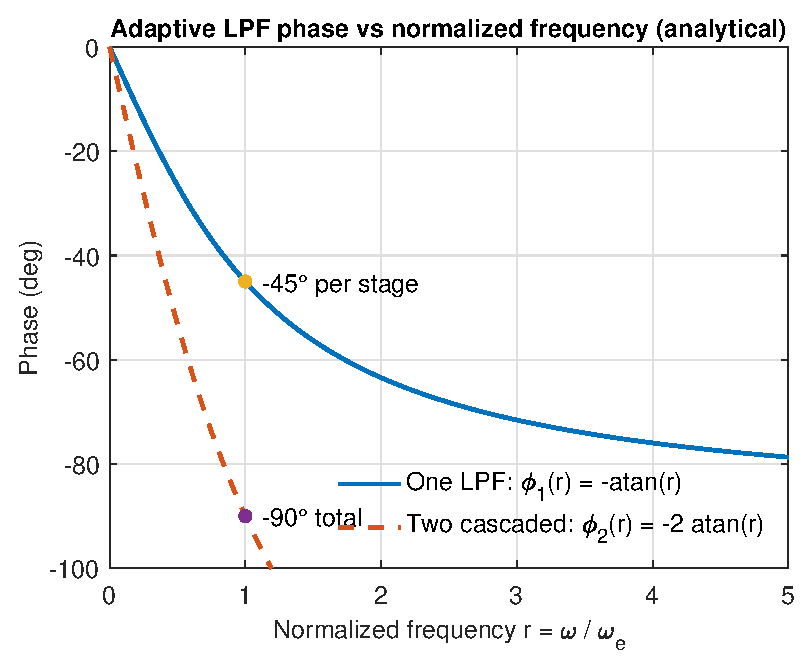
\includegraphics[width=\textwidth]{./Filter}
	\caption{Cascaded First Order Filter Response}
	\label{fig:FilterResponse}
\end{figure}

Let the switching action be
\[
\mathbf s = \eta_0\,
\begin{bmatrix}
	\operatorname{sgn}(\tilde i_\alpha) \\ 
	\operatorname{sgn}(\tilde i_\beta)
\end{bmatrix}.
\]

The cascaded filters are
\begin{equation}
	\label{eq:smo-lpf1}
	\dot{\mathbf z}_1 = -2\pi\, f_c(\omega_e)\, \mathbf z_1 + 2\pi\, f_c(\omega_e)\, \mathbf s ,
\end{equation}
\begin{equation}
	\label{eq:smo-lpf2}
	\dot{\mathbf z}_2 = -2\pi\, f_c(\omega_e)\, \mathbf z_2 + 2\pi\, f_c(\omega_e)\, \mathbf z_1 ,
\end{equation}
\begin{equation}
	\label{eq:smo-ehat-cascade}
	\begin{bmatrix} \hat e_\alpha \\ \hat e_\beta \end{bmatrix} = \mathbf z_2 .
\end{equation}
The speed-scheduled cutoff is
\begin{equation}
	\label{eq:smo-fc-omega}
	f_c(\omega_e) = \operatorname{clip}\!\Big( \tfrac{|\omega_e|}{2\pi} ,\; f_{\min} ,\; \min\{ f_{\max} ,\, f_{\mathrm{PWM}}/10 \} \Big) .
\end{equation}


% =====================================================================
% Subsection: Speed Estimation from Estimated Electrical Angle
% Context: angle \hat\theta_e is available from atan2 on the back-EMF vector
% Policy: minimal inline math; key formulas displayed and labeled
% Requires: \usepackage{amsmath,amssymb}
% =====================================================================

% =====================================================================
% Subsection: Speed Estimation from Estimated Electrical Angle — Simple 1st-Order LPF
% Replaces the previous smoothing (Tustin) with a single-coefficient recursion
% Requires: \usepackage{amsmath,amssymb}
% =====================================================================

\subsection{Speed Estimation from the Estimated Electrical Angle}
\label{subsec:speed-from-angle-simple}


This subsection computes electrical and mechanical speed from the estimated electrical angle obtained via the arctangent of the back-EMF vector. A plain differentiator is used, followed by a simple first-order low-pass filter applied only to the speed.


The estimator assumes a uniformly sampled angle sequence with sampling period shown in \eqref{eq:spdS-Ts}.
\begin{equation}
	\label{eq:spdS-Ts}
	T_s > 0 .
\end{equation}
The wrapped electrical angles are denoted in \eqref{eq:spdS-theta}.
\begin{equation}
	\label{eq:spdS-theta}
	\hat\theta_e[k] \in (-\pi,\,\pi] ,\qquad k=0,1,2,\dots
\end{equation}


Let the raw sample–to–sample angle difference be
\begin{equation}
	\label{eq:spd-dtheta-raw}
	\Delta\theta_{\mathrm{raw}}[k] = \hat\theta_e[k] - \hat\theta_e[k-1] .
\end{equation}
To suppress the $\pm 2\pi$ wrap, compare $\Delta\theta_{\mathrm{raw}}[k]$ with a limit
$\Delta\theta_{\lim}\in(\tfrac{\pi}{2},\,\pi]$ and correct as
\begin{equation}
	\label{eq:spd-dtheta-limited}
	\Delta\theta_e[k] =
	\begin{cases}
		\Delta\theta_{\mathrm{raw}}[k] - 2\pi, & \Delta\theta_{\mathrm{raw}}[k] > \Delta\theta_{\lim},\\[4pt]
		\Delta\theta_{\mathrm{raw}}[k] + 2\pi, & \Delta\theta_{\mathrm{raw}}[k] < -\,\Delta\theta_{\lim},\\[4pt]
		\Delta\theta_{\mathrm{raw}}[k], & \text{otherwise.}
	\end{cases}
\end{equation}
The electrical speed estimate then is
\begin{equation}
	\label{eq:spd-omega-from-dtheta}
	\hat\omega_e[k] = \frac{\Delta\theta_e[k]}{T_s}.
\end{equation}
the sampling period satisfies
\begin{equation}
	\label{eq:spd-sampling-bound}
	T_s < \frac{\Delta\theta_{\lim}}{\omega_{e,\max}}
	\quad\Big(\text{equivalently } f_s > \omega_{e,\max}/\Delta\theta_{\lim}\Big),
\end{equation}
so that genuine inter-sample motion never exceeds the limit and only wrap events are corrected.



The raw electrical speed estimate is then
\begin{equation}
	\label{eq:spdS-omega-raw}
	\hat\omega_e[k] = \frac{\Delta\theta_e[k]}{T_s} .
\end{equation}


The raw speed \(\hat\omega_e[k]\) is smoothed by a single-coefficient recursion as in \eqref{eq:spdS-simple-lpf}. This is the discrete first-order low-pass filter you requested ("\(Y[k]=G\,Y[k-1]+(1-G)U[k]\)") with input \(U[k]=\hat\omega_e[k]\) and output \(Y[k]=\omega_{e,f}[k]\).
\begin{equation}
	\label{eq:spdS-simple-lpf}
	\omega_{e,f}[k] = G\; \omega_{e,f}[k-1] + (1-G)\; \hat\omega_e[k] .
\end{equation}
Two equivalent expressions for the filter coefficient are commonly used:
\begin{equation}
	\label{eq:spdS-G-exact}
	G = e^{-\omega_c T_s} ,
\end{equation}
\begin{equation}
	\label{eq:spdS-G-approx}
	G \approx \frac{1}{1 + \omega_c T_s} \quad \text{for small } \omega_c T_s .
\end{equation}
Equation \eqref{eq:spdS-G-exact} is the exact zero-order-hold discretization of a first-order lag with cutoff \(\omega_c\); Equation \eqref{eq:spdS-G-approx} is a convenient algebraic approximation giving nearly identical factors when \(\omega_c T_s\ll 1\).

Mechanical speed and revolutions per minute follow from \eqref{eq:spdS-omegam} and \eqref{eq:spdS-rpm} using the number of pole pairs \(p\).
\begin{equation}
	\label{eq:spdS-omegam}
	\hat\omega_m[k] = \frac{\omega_{e,f}[k]}{p} .
\end{equation}
\begin{equation}
	\label{eq:spdS-rpm}
	\hat n[k] = \frac{60}{2\pi} \, \hat\omega_m[k] .
\end{equation}


% =====================================================================
% Subsection: PI Field-Oriented Speed Controller — Pole-Placement Design
% Context: SPMSM, i_d ≈ 0, fast inner current loops (i_q tracking ≈ ideal)
% Requires: \usepackage{amsmath,amssymb}
% Policy: keep equations displayed and labeled; prose explains each step
% =====================================================================

% =====================================================================
% Subsection: FOC Speed PI via Pole Placement (Series topology C(s)=k_p(1+k_i/s))
% Requires: \usepackage{amsmath,amssymb}
% =====================================================================

% =====================================================================
% Subsection: PI Speed Controller by Pole Cancellation (Series topology)
% Requires: \usepackage{amsmath,amssymb}
% =====================================================================

% =====================================================================
% Subsection: Series PI Speed Controller by Pole Cancellation (Design Story)
% Requires: \usepackage{amsmath,amssymb}
% =====================================================================

\section{Transfer functions and System Parameters}
\label{subsec:Transfer-Functions}
\subsection{Series PI Current Controller by Pole Cancellation}
\label{subsec:pi-current-series-pc}


For control design and analysis, the inverter is represented by an average model over each PWM period. After using decoupling due to presence of $\omega$L terms, equations \eqref{eq:narr-dq-vd} and \eqref{eq:narr-dq-vq} can be decoupled as follows:

\begin{equation}
	\label{eq:idcurr-dq}
	L\frac{\mathrm d i_d}{\mathrm d t} = (R\, + Rce) i_d + v^{*}_{d}.
\end{equation}

\begin{equation}
	\label{eq:iqcurr-dq}
	L\frac{\mathrm d i_q}{\mathrm d t} = (R\, + Rce) i_q + v^{*}_{q}.
\end{equation}

Where $v^{*}_{d}$ and $v^{*}_{q}$ can be described as the voltage references which represent the PI control actions in the synchronous dq reference frame from which the grid currents $id$ and $iq$ can be controlled.

From equations \eqref{eq:narr-dq-vd} and \eqref{eq:narr-dq-vq}, the transfer function of the inner current loops for the grid currents can be expressed in Laplace Domain in the synchronous dq frame as follows:

\begin{equation}
	\label{eq:cur-Gp}
	G_i(s) \;=\; \frac{I(s)}{U(s)} \;=\; \frac{1}{L\, s + (R\, + Rce)} .
\end{equation}

Use the series PI topology on both axes:
\begin{equation}
	\label{eq:cur-C}
	C(s) \;=\; k_p \left( 1 + \frac{k_i}{s} \right) \;=\; k_p\,\frac{s + k_i}{s} .
\end{equation}
Place the controller zero on the plant pole:
\begin{equation}
	\label{eq:curr-cancell}
	k_i \;=\; \frac{R}{L} .
\end{equation}
With \eqref{eq:curr-cancell}, the loop reduces to a pure integrator gain:
\begin{equation}
	\label{eq:cur-loop}
	L(s) \;=\; C(s)\,G_i(s) \;=\; \frac{k_p}{L}\,\frac{1}{s} .
\end{equation}

Select the desired closed-loop bandwidth (per axis):
\begin{equation}
	\label{eq:cur-wc}
	\omega_{ci} \;>\; 0 , \qquad \tau_i \;=\; \frac{1}{\omega_{ci}} .
\end{equation}
The proportional gain that realizes \eqref{eq:cur-wc} is
\begin{equation}
	\label{eq:cur-kp}
	k_p \;=\; L\, \omega_{ci} \;=\; \frac{L}{\tau_i} .
\end{equation}
Equations \eqref{eq:curr-cancell}–\eqref{eq:cur-kp} produce a first-order, monotonic current response with zero steady-state error to step references (neglecting saturation).


For each axis, define the error, the integrator state, and the auxiliary control:
\begin{equation}
	\label{eq:cur-realize}
	e_d = i_d^{\ast} - i_d , \qquad \dot{x}_{I,d} = k_i\, e_d , \qquad u_d = k_p\,(e_d + x_{I,d}) ,
\end{equation}
\begin{equation}
	\label{eq:cur-realize-q}
	e_q = i_q^{\ast} - i_q , \qquad \dot{x}_{I,q} = k_i\, e_q , \qquad u_q = k_p\,(e_q + x_{I,q}) .
\end{equation}
Recover the commanded dq voltages for the PWM modulator:
\begin{equation}
	\label{eq:cur-vdcmd}
	v_d^{\ast} \;=\; u_d \;-\; \omega_e\, L_s\, i_q ,
\end{equation}
\begin{equation}
	\label{eq:cur-vqcmd}
	v_q^{\ast} \;=\; u_q \;+\; \omega_e\, L_s\, i_d .
\end{equation}


Limit the voltage vector to the available DC bus (space-vector circle limitation):
\begin{equation}
	\label{eq:cur-sat}
	\begin{bmatrix} v_d^{\ast\,\mathrm{sat}} \\[2pt] v_q^{\ast\,\mathrm{sat}} \end{bmatrix}
	= \operatorname{sat}_{V_{\max}}\!\left( \begin{bmatrix} v_d^{\ast} \\ v_q^{\ast} \end{bmatrix} \right) ,
	\qquad V_{\max} \approx \frac{V_{\mathrm{dc}}}{\sqrt{3}} .
\end{equation}
Apply back-calculation anti-windup on each axis using the voltage deficit:
\begin{equation}
	\label{eq:cur-aw-d}
	\dot{x}_{I,d} \;=\; k_i\, e_d \;+\; \frac{K_{aw}}{k_p}\,\big( v_d^{\ast\,\mathrm{sat}} - v_d^{\ast} \big) ,
\end{equation}
\begin{equation}
	\label{eq:cur-aw-q}
	\dot{x}_{I,q} \;=\; k_i\, e_q \;+\; \frac{K_{aw}}{k_p}\,\big( v_q^{\ast\,\mathrm{sat}} - v_q^{\ast} \big) .
\end{equation}


The $d$- and $q$-axis series PI controllers are tuned by pole cancellation, placing the controller zero at the plant pole and using the proportional gain to set a first-order closed-loop pole. With $L=0.018585~\mathrm{H}$ and $R = 0.55~\Omega$, and choosing a closed-loop bandwidth of $f_{ci}=100~\mathrm{Hz}$ as shown in \ref{fig:CurrentControllerBodePlot},
\begin{equation}
	\label{eq:cur-wci-num}
	\omega_{ci} = 2\pi\cdot 100 = 628.31853~\text{rad/s}, \qquad \tau_i=\frac{1}{\omega_{ci}}=1.5915\times 10^{-3}~\text{s},
\end{equation}
\begin{equation}
	\label{eq:cur-ki-num}
	k_{i,d}=k_{i,q}=\frac{R_s}{L}=\frac{0.55}{0.018585}=29.594~\text{rad/s},
\end{equation}
\begin{equation}
	\label{eq:cur-kp-num}
	k_{p,d}=k_{p,q}=L\,\omega_{ci}=0.018585\times 628.31853=11.677~.
\end{equation}
This yields identical first-order closed-loop dynamics on both axes with time constant $\tau_i\approx1.5915$\,ms and zero steady-state error to step current commands. (If a different $f_{ci}$ is adopted, recompute only $k_{p,\{\!d,q\!\}}=L\,\omega_{ci}$ while keeping $k_{i,\{\!d,q\!\}}=R/L$.)

\begin{figure}[H]
	\centering
	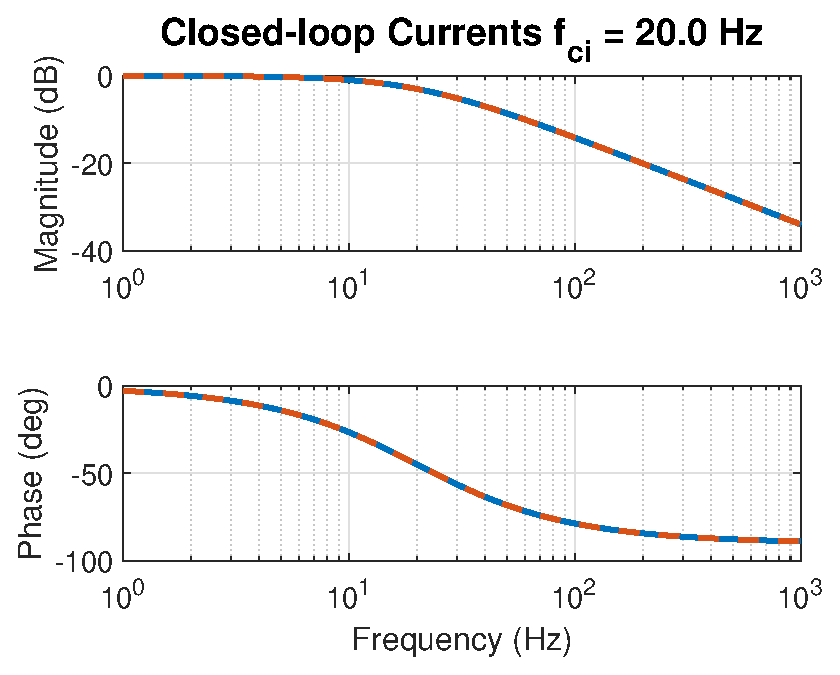
\includegraphics[width=\textwidth]{./CurrentControllerBodePlot}
	\caption{DQ-Axes Controller Design Bode Plot}
	\label{fig:CurrentControllerBodePlot}
\end{figure}

\subsection{Series PI DC-Link Voltage Controller by Pole Cancellation}
\label{subsec:pi-vdc-series-pc}


The outer DC-Link Voltage loop commands the direct–current reference so that the DC-Link Voltage requested by the load tracks its reference. The inner current loops are assumed fast, therefore the direct current tracks its command with negligible dynamics. A series PI is adopted and tuned to have narrower bandwidth (or slower time constant) than the current loop.

By using the balance for the active power given in \eqref{eq:narr-pe}: 
\begin{equation}
	\label{eq:pc-dc}
	\hat{P} = V_{sd}\hat{I_{d}} + V_{sq}\hat{I_{q}} +\tfrac{L}{2}\,\tfrac{d(\hat{I_{d}^2}+\hat{I_{q}^2})}{dt}\ = \tfrac{C}{2}\,\tfrac{d(\hat{V_{dc}^2})}{dt}\ + \hat{V_{dc}}I_{dc} 
\end{equation}

The transfer function between the DC-Link voltage and the grid current in D-axis can be derived from \eqref{eq:pc-dc} as follows:
\begin{equation}
	\label{eq:pc-Gvdc}
	G_{d}(s) = \tfrac{\hat{Vdc}}{\hat{Id}} = \tfrac{-sLId+V_{sd}}{sCV_{dc}+I_{dc}}.
\end{equation}

The series PI is written as
\begin{equation}
	\label{eq:pc-controller}
	C(s) = k_p\!\left(1 + \frac{k_i}{s}\right) = k_p\,\frac{s + k_i}{s} .
\end{equation}
%The controller zero is placed to cancel the plant pole by setting
%\begin{equation}
%	\label{eq:pc-cancel}
%	k_i = \frac{B}{J} .
%\end{equation}
With \eqref{eq:pc-Gvdc}, the loop gain with voltage transfer function has 2 poles and a RHP zero. 

The closed loop from DC-Link Voltage reference reduces to first order by the assumption of fast inner current loop.

The speed loop bandwidth and time constant are chosen explicitly as
\begin{equation}
	\label{eq:pc-wc}
	\omega_c > 0 , \qquad \tau = \frac{1}{\omega_c} .
\end{equation}

Define the speed error and the PI internal state and torque command as
\begin{equation}
	\label{eq:pc-realize}
	e_{V_{dc}} = V_{dcref}^{*} - V_{dc}.
\end{equation}
The direct–current command follows from the control action of the outer DC-Link Voltage. The commanded current is limited to the available range:

\begin{equation}
	\label{eq:pc-sat}
	i_d^{\ast\,\mathrm{sat}} = \operatorname{sat}\!\big(i_d^{\ast};\, -i_{d,\max},\, i_{d,\max}\big).
\end{equation}

In this work, the series PI speed controller is tuned for a closed-loop bandwidth of 10\,Hz as shown in Figure\ref{fig:SpeedControllerBodePlot}, ensuring clear separation from the inner current loops while preserving ripple free DC-Link Voltage. Using the pole-cancellation design, the controller zero is placed at the mechanical pole and the proportional gain sets the first-order closed-loop pole. The design values are:
\begin{equation}
	\label{eq:speed-wc-num}
	\omega_c = 2\pi\cdot 10 = 62.832~\text{rad/s}, \qquad \tau=\frac{1}{\omega_c}=0.01592~\text{s},
\end{equation}
%\begin{equation}
%	\label{eq:kt-num}
%	K_t = \tfrac{3}{2}\,p\,\lambda_f = \tfrac{3}{2}\cdot 4 \cdot 0.1227 = 0.7362~\text{N\,m/A},
%\end{equation}
\begin{equation}
	\label{eq:ki-num}
	k_i = 1.5~\text{rad/s},
\end{equation}
\begin{equation}
	\label{eq:kp-num}
	k_p = 0.25.
\end{equation}
With \(k_i\) and \(k_p\) as above, the closed-loop speed response is first-order with time constant \(\tau\approx 0.0159\) s and zero steady-state error to step commands with proper dynamics with a suitable bandwidth from the bandwidth of the current controllers.

\begin{figure}[h]
	\centering
	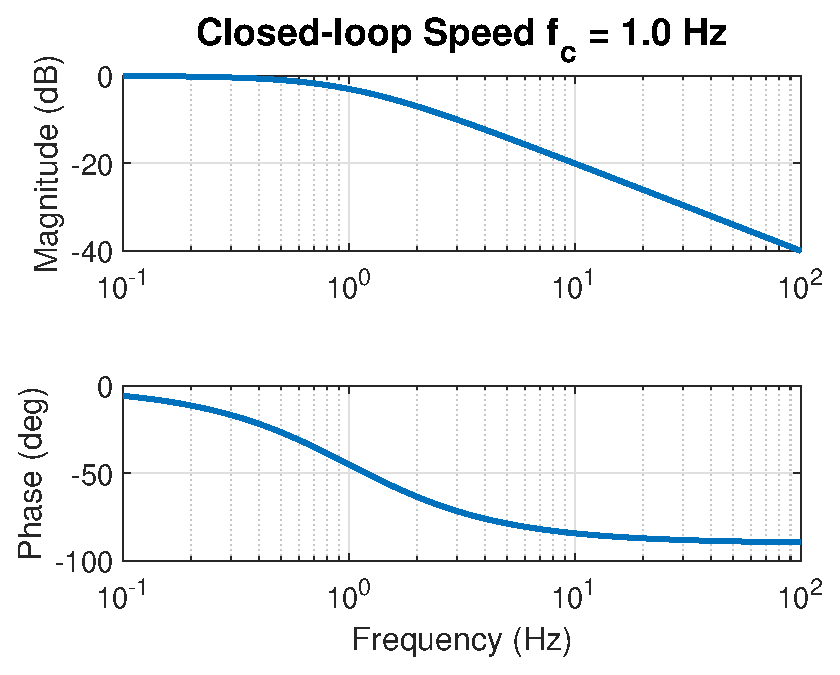
\includegraphics[width=\textwidth]{./SpeedControllerBodePlot}
	\caption{Speed Controller Design Bode Plot}
	\label{fig:SpeedControllerBodePlot}
\end{figure}
% =====================================================================
% Subsection: Series PI dq-Current Controllers by Pole Cancellation
% Context: SPMSM (L_d=L_q=L_s), sensorless-ready; inner loops much faster than speed loop
% Requires: \usepackage{amsmath,amssymb}
% =====================================================================



\section{Modeling and Simulations}
This section validates the complete drive model and controllers through a focused suite of studies: (i) steady-state operation to verify ripple, losses, and harmonic content; (ii) low-speed operation to probe back-EMF limits and non-idealities; (iii)  dynamic performance under speed/current steps; (iv) parameter variation to gauge robustness against model mismatch; and (v) load variation to assess torque disturbance rejection.

\subsection{Steady State Operation}
Under an ideal plant/inverter (no non-linearities or disturbances), the sensorless PI drive holds 1000 rpm (50\% of rated) with clean steady-state behavior at both load points: at low load (10\% rated torque, \(0.3~\mathrm{N\,m}\)) the phase-current THD is \(\mathbf{0.8\%}\) (see Fig.~\ref{fig:PIIdeal_1000rpm_low}), and at medium load (50\% rated torque, \(1.75~\mathrm{N\,m}\)) it remains \(\mathbf{0.8\%}\) (see Fig.~\ref{fig:PIIdeal_1000rpm_med}). The identical THD across torques indicates that—absent inverter distortions—the harmonic floor is set by discretization/modulation rather than load, while speed regulation stays tight and ripple minimal.

% Requires in preamble:
% \usepackage{graphicx}
% \usepackage{subcaption}

\begin{figure}[H]
  \centering
  \begin{subfigure}{0.485\textwidth}
    \centering
    % Replace with your exported plot/image
    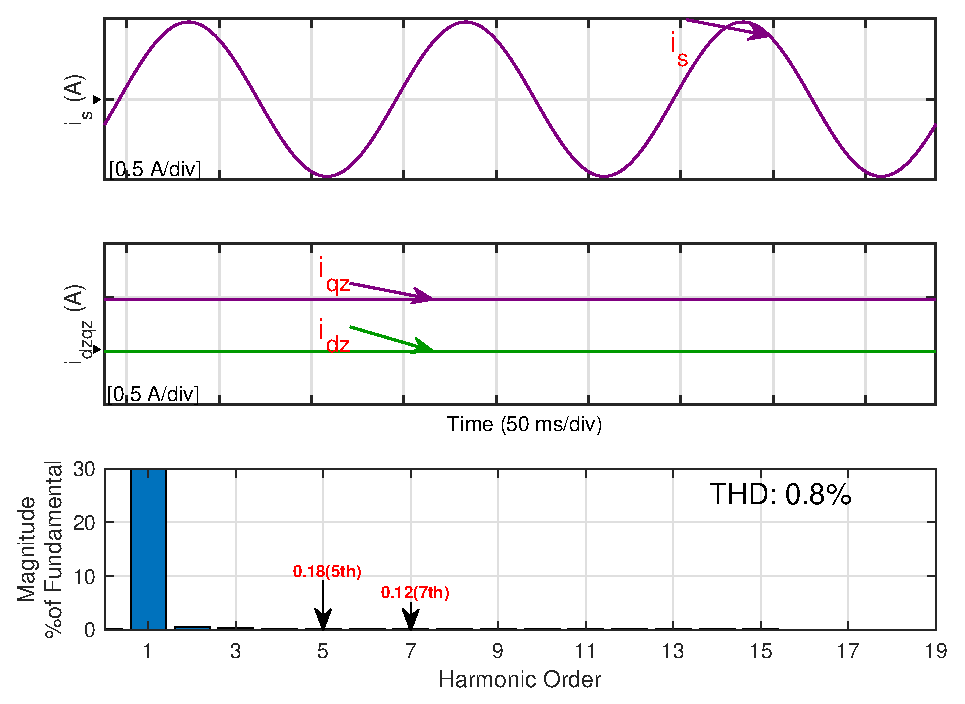
\includegraphics[width=\linewidth]{./MidSpeedLowLoadSteadyState}
    \caption{Low load: \(T=0.3~\mathrm{N\,m}\), \\THD \(=0.8\%\).}
    \label{fig:PIIdeal_1000rpm_low}
  \end{subfigure}\hfill
  \begin{subfigure}{0.485\textwidth}
    \centering
    % Replace with your exported plot/image
    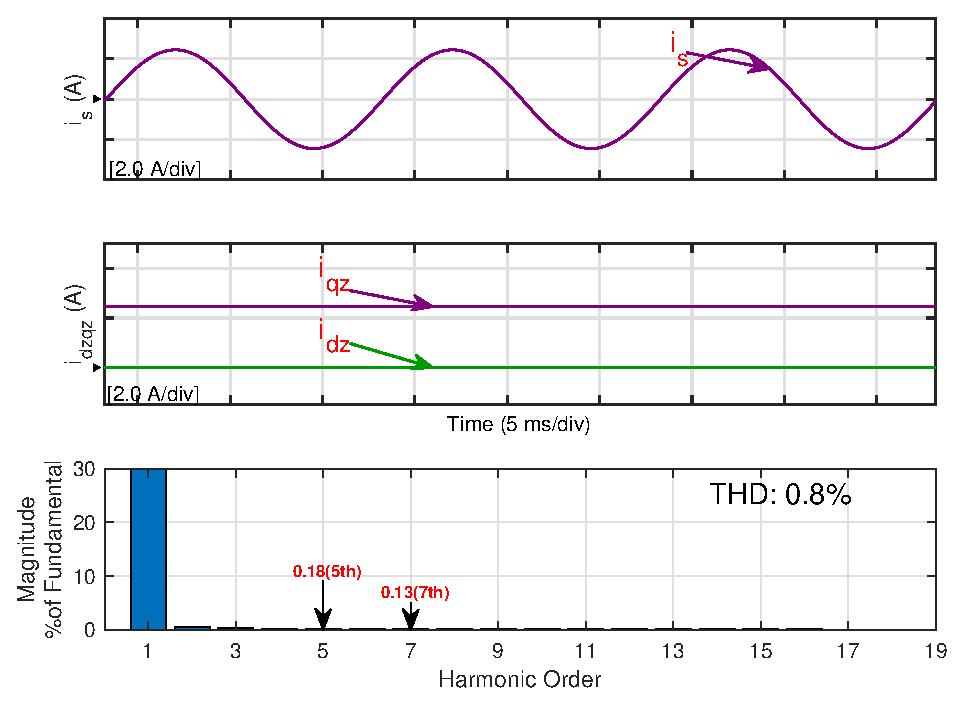
\includegraphics[width=\linewidth]{./MidSpeedMidLoadSteadyState}
    \caption{Medium load: \(T=1.75~\mathrm{N\,m}\),\\ THD \(=0.8\%\).}
    \label{fig:PIIdeal_1000rpm_med}
  \end{subfigure}
  \caption{PI controller steady state at 50\% rated speed (1000 rpm, ideal model). Each panel shows phase current, \(i_{dq}\), and THD.}
  \label{fig:PIIdeal_1000rpm}
\end{figure}


\subsection{Unbalanced Grid Operation}
With an ideal plant/inverter model (no non-linearities or disturbances), the sensorless PI drive maintains accurate low-speed control across load extremes. At 5\% of rated speed (100~rpm), the phase-current THD is \(\mathbf{1.3\%}\) at low load (10\% rated torque, \(0.3~\mathrm{N\!\cdot\!m}\)) and \(\mathbf{0.3\%}\) at high load (100\% rated torque, \(3.5~\mathrm{N\!\cdot\!m}\)); see Fig.~\ref{fig:PIIdeal_100rpm}. At 10\% of rated speed (200~rpm), the THD is \(\mathbf{1.6\%}\) at \(0.3~\mathrm{N\!\cdot\!m}\) and again \(\mathbf{0.3\%}\) at \(3.5~\mathrm{N\!\cdot\!m}\); see Fig.~\ref{fig:PIIdeal_200rpm}. In both tests the tracking is tight and ripple modest; the lower THD at higher load reflects stronger EMF/current improving the sensorless angle estimation and reducing relative harmonic content. Overall, these ideal-simulation results evidence robust PI performance at low speeds under all tested loads.

% Requires in preamble:
% \usepackage{graphicx}
% \usepackage{subcaption}
% (Optional) \usepackage{siunitx}

% ---------- Fig: PI at 5% rated (100 rpm) ----------
\begin{figure}[H]
  \centering
  \begin{subfigure}{0.485\textwidth}
    \centering
    % Replace with your exported plot/image
    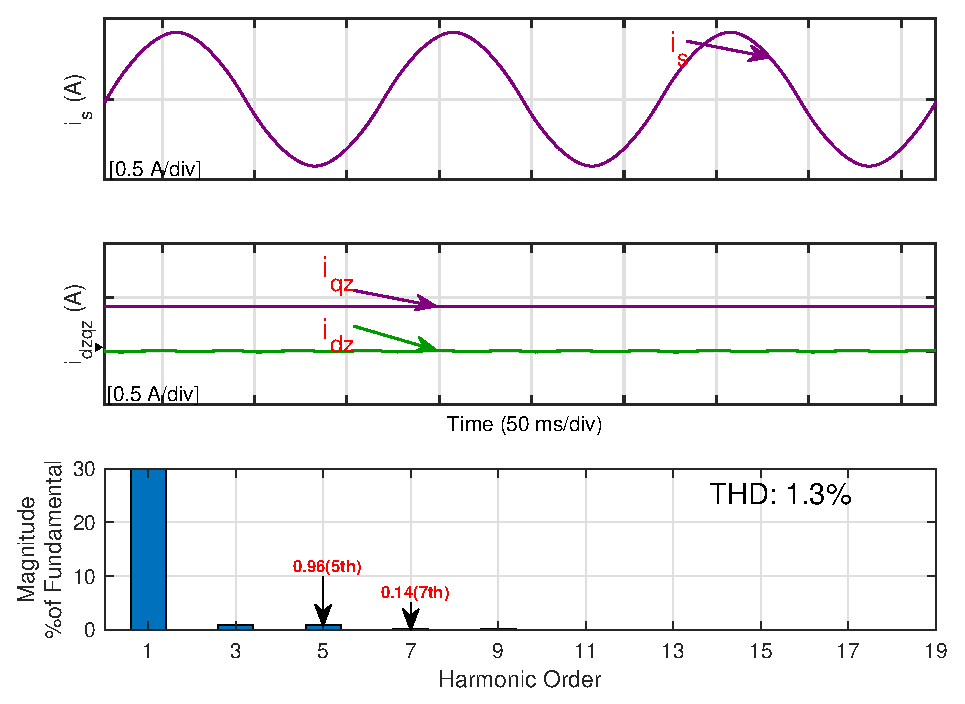
\includegraphics[width=\linewidth]{./PISteadyStateLowLoad100Rpm}
    \caption{Low load: \(T=0.3~\mathrm{N\,m}\), THD \(=1.3\%\).}
    \label{fig:PIIdeal_100rpm_low}
  \end{subfigure}\hfill
  \begin{subfigure}{0.485\textwidth}
    \centering
    % Replace with your exported plot/image
    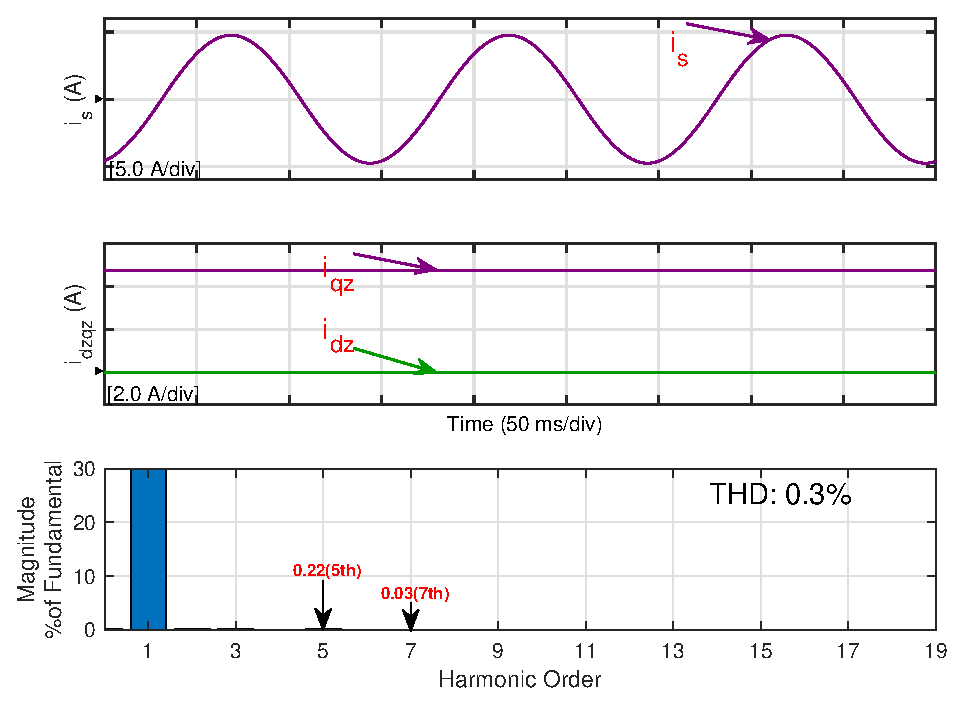
\includegraphics[width=\linewidth]{./PISteadyStateHighLoad100Rpm}
    \caption{High load: \(T=3.5~\mathrm{N\,m}\), THD \(=0.3\%\).}
    \label{fig:PIIdeal_100rpm_high}
  \end{subfigure}
  \caption{PI controller at 5\% rated speed (100 rpm, ideal model). Each panel shows phase current, \(i_{dq}\), and THD.}
  \label{fig:PIIdeal_100rpm}
\end{figure}

% ---------- Fig: PI at 10% rated (200 rpm) ----------
\begin{figure}[H]
  \centering
  \begin{subfigure}{0.485\textwidth}
    \centering
    % Replace with your exported plot/image
    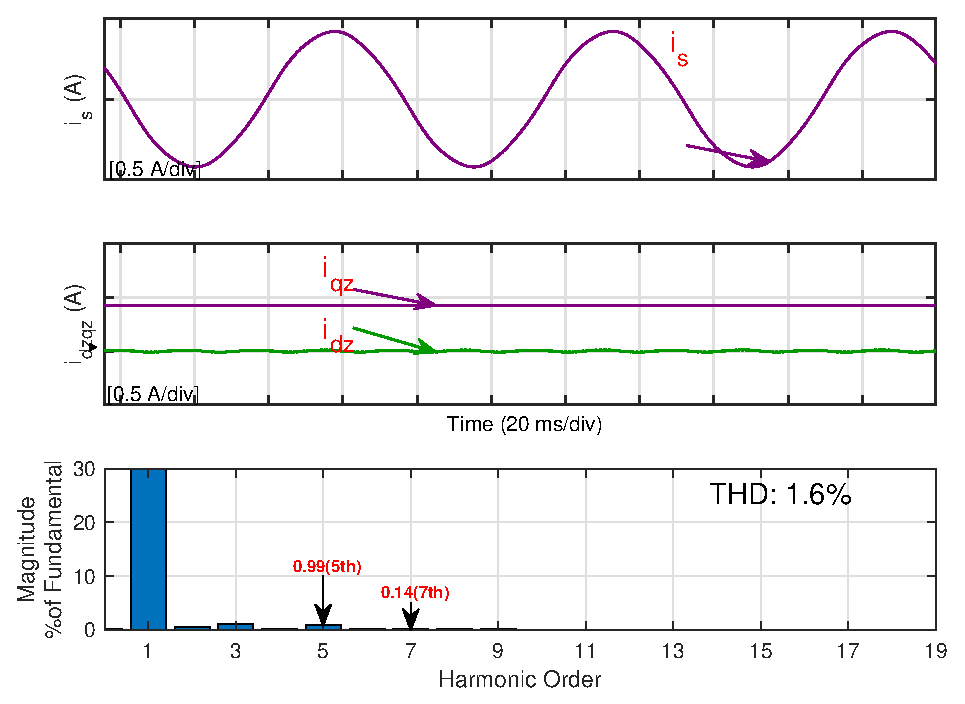
\includegraphics[width=\linewidth]{./PISteadyStateLowLoad200Rpm}
    \caption{Low load: \(T=0.3~\mathrm{N\,m}\), THD \(=1.6\%\).}
    \label{fig:PIIdeal_200rpm_low}
  \end{subfigure}\hfill
  \begin{subfigure}{0.485\textwidth}
    \centering
    % Replace with your exported plot/image
    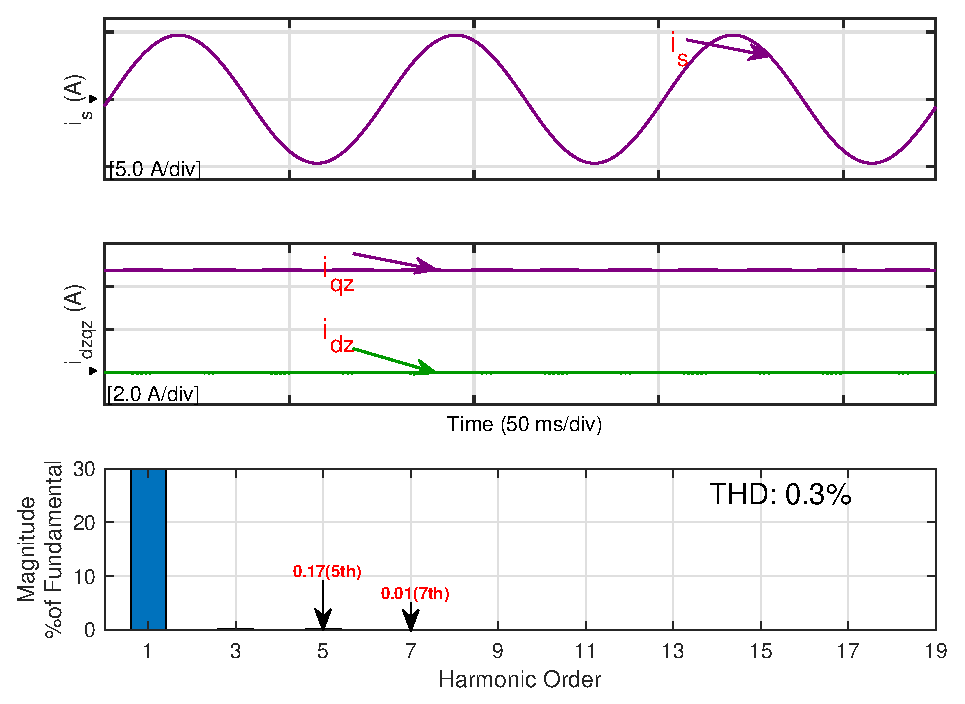
\includegraphics[width=\linewidth]{./PISteadyStateHighLoad200Rpm}
    \caption{High load: \(T=3.5~\mathrm{N\,m}\), THD \(=0.3\%\).}
    \label{fig:PIIdeal_200rpm_high}
  \end{subfigure}
  \caption{PI controller at 10\% rated speed (200 rpm, ideal model). As in the 100 rpm case, speed and currents remain well behaved; higher load yields lower relative harmonic content.}
  \label{fig:PIIdeal_200rpm}
\end{figure}

\subsection{Dynamic Performance}
Under an ideal plant/inverter (no non-linearities or disturbances), the PI speed loop tracks set-point changes within the 10–50\% band (100~rpm \(\rightarrow\) 1000~rpm) cleanly at both load extremes. At \emph{low load} (10\% rated torque, \(0.3~\mathrm{N\,m}\)), the measured speed follows the command with overshoot \(\mathbf{<10\%}\) and negligible steady-state error (see Fig.~\ref{fig:PIDyn_100to1000_low}). At \emph{rated load} (\(3.5~\mathrm{N\,m}\)), the response is slightly slower but remains well damped with overshoot \(\mathbf{<10\%}\) and zero steady-state error (see Fig.~\ref{fig:PIDyn_100to1000_rated}). These results confirm robust and smooth dynamic behavior across the tested range.

% Requires in preamble:
% \usepackage{graphicx}
% \usepackage{subcaption}

\begin{figure}[H]
  \centering
  \begin{subfigure}{0.485\textwidth}
    \centering
    % Replace with your exported plot/image
    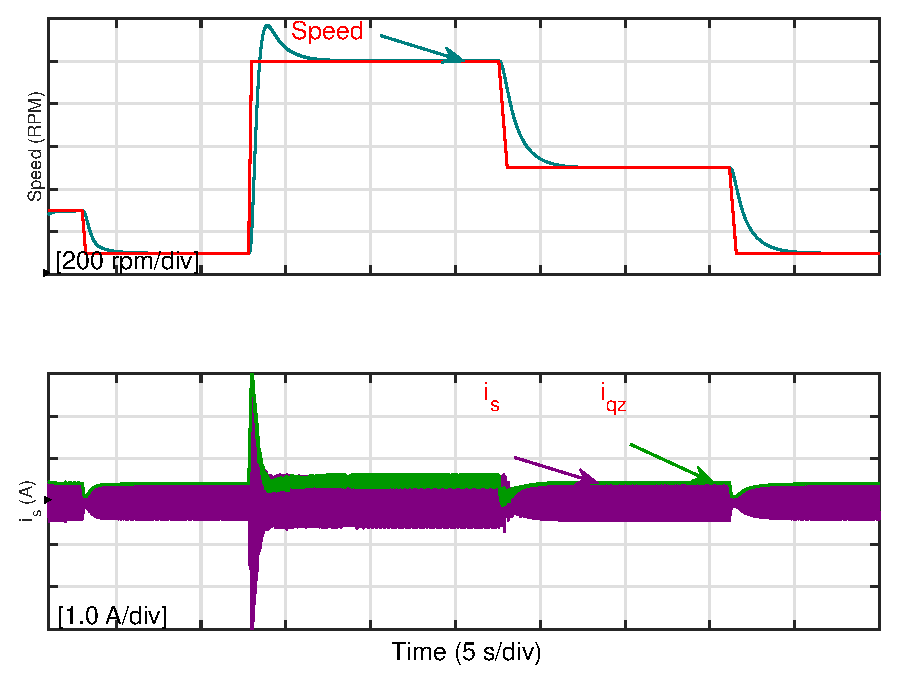
\includegraphics[width=\linewidth]{./DynamicResponsePILowLoad}
    \caption{Low load: \(T=0.3~\mathrm{N\,m}\). Overshoot \(<10\%\); zero steady-state error.}
    \label{fig:PIDyn_100to1000_low}
  \end{subfigure}\hfill
  \begin{subfigure}{0.485\textwidth}
    \centering
    % Replace with your exported plot/image
    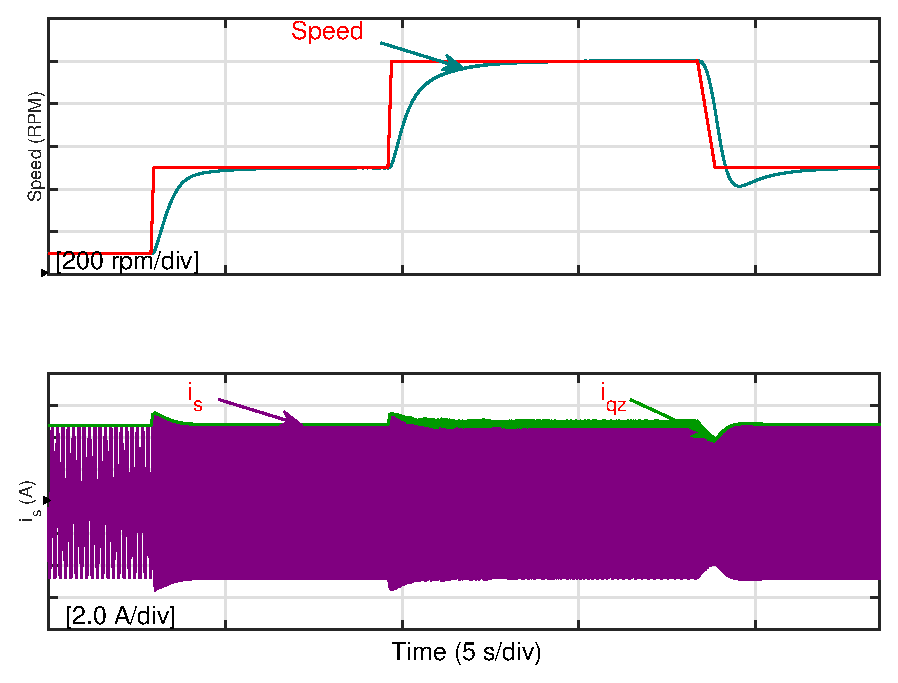
\includegraphics[width=\linewidth]{./DynamicResponsePIHighLoad}
    \caption{Rated load: \(T=3.5~\mathrm{N\,m}\). Slightly slower, well-damped; overshoot \(<10\%\).}
    \label{fig:PIDyn_100to1000_rated}
  \end{subfigure}
  \caption{PI controller dynamic response (ideal model) for speed changes within the \(10\%\!\to\!50\%\) rated band (100~rpm to 1000~rpm). Each panel shows command vs.\ speed, \(i_q\), and phase currents.}
  \label{fig:PIDyn_100to1000}
\end{figure}


\subsection{Parameter Variation}
In the ideal (noise-/nonlinearity-free) simulation, the PI controller was exercised with a deliberately biased motor model: \(R_s\) increased by \(+25\%\) and \(L_{d,q}\) decreased by \(25\%\). This shifts the electrical time constant from \(\tau=L/R\) to \(\tau'=\tfrac{0.75L}{1.25R}=0.60\,\tau\), moving the plant pole right and nudging the closed-loop cutoff upward while preserving phase margin. At the worst case examined—5\% rated speed (100~rpm)—the phase-current THD rises modestly from \(\mathbf{1.3\%}\) to \(\mathbf{1.7\%}\), but speed tracking and settling remain essentially unchanged. As illustrated in Fig.~\ref{fig:PIParameterVariation} (phase current, \(dq\) currents, and THD), the small THD increase reflects the altered crossover and slight model–controller mismatch; with no inverter non-idealities or disturbances, there is no mechanism to amplify it, so PI performance stays robust.
% Requires in preamble:
% \usepackage{graphicx}
% \usepackage{subcaption}

\begin{figure}[H]
  \centering
  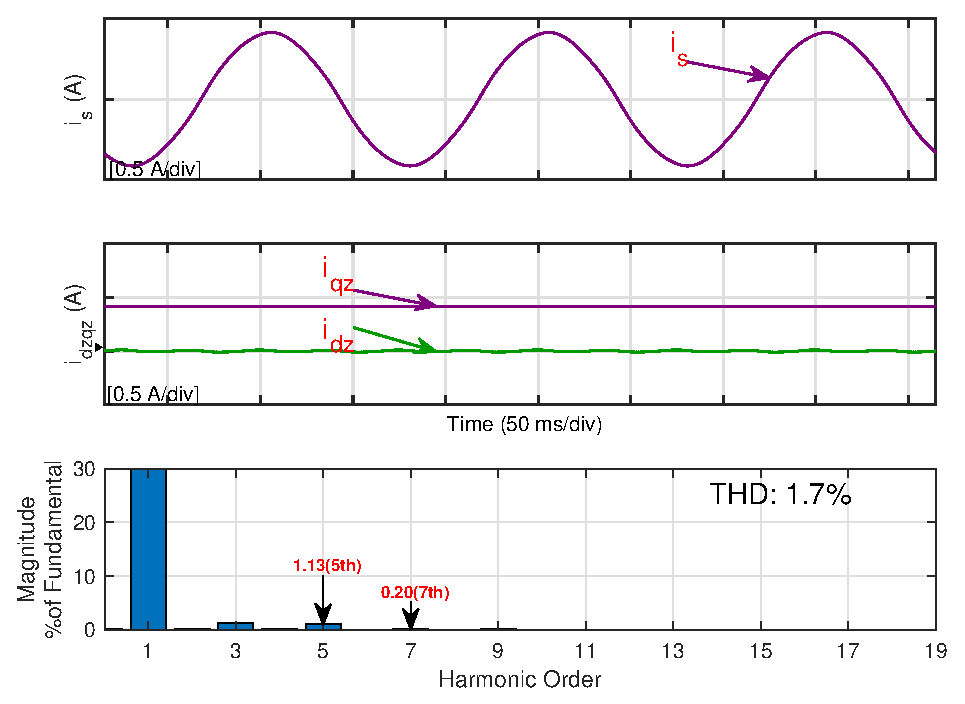
\includegraphics[width=0.485\linewidth]{./ParameterVariation}
  \caption{PI controller—parameter variation at 5\% rated speed (100 rpm, ideal model). The motor model is perturbed with \(R_s{+}25\%\) and \(L_{d,q}{-}25\%\). Panels show (a) phase current overlay, (b) \(dq\) currents, and (c) THD comparison.}
  \label{fig:PIParameterVariation}
\end{figure}



\subsection{Load Variation}
At 1000 rpm, the torque load was swept from 10\% to 100\% of rated in 20\% increments, each plateau held to steady state. As shown in Fig.~\ref{fig:PILoadVariation}, the PI loop maintains the commanded speed with small, well-damped transients at each step; \(i_q\) increases in clean steps to furnish torque and the phase currents scale proportionally without oscillation. Figure~\ref{fig:PILoadVariation} thus evidences robust disturbance rejection and steady regulation across the entire load range under ideal conditions.

% Requires in preamble:
% \usepackage{graphicx}
% \usepackage{subcaption}

\begin{figure}[H]
  \centering
  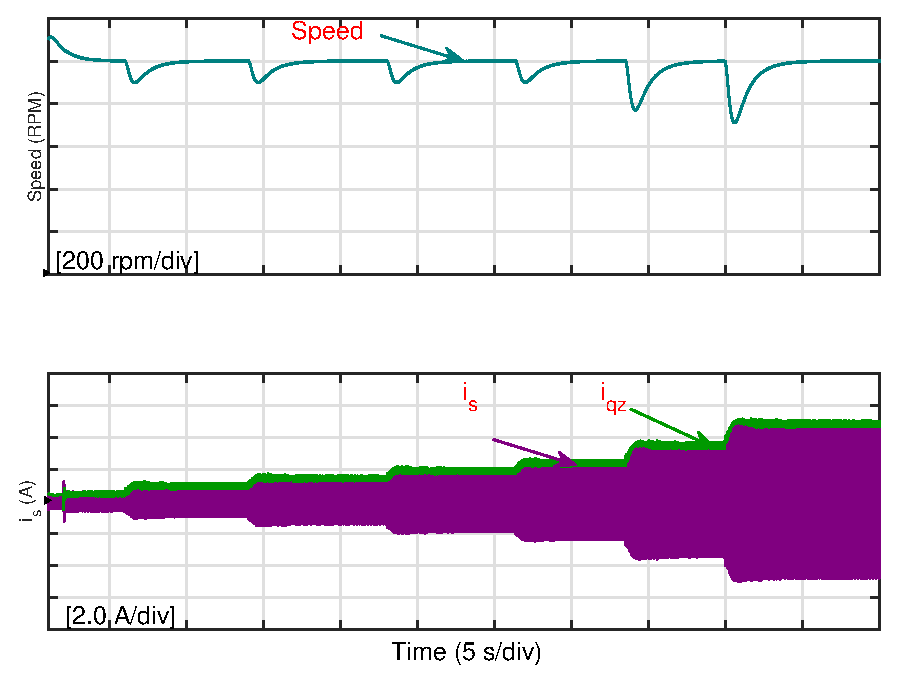
\includegraphics[width=0.6\linewidth]{./LoadVariation}
  \caption{PI controller under load variation at 50\% rated speed (1000 rpm, ideal model). The load torque steps from 10\% to 100\% in 20\% increments.}
  \label{fig:PILoadVariation}
\end{figure}

% =====================================================================
% Subsection: Motor and Drive Parameters (Comprehensive Table)
% Requires in preamble: \usepackage{longtable,booktabs}
% Optional: \usepackage{siunitx} for neat units
% =====================================================================



% End of subsection




% Notes: choose f_{T,min} just above current-loop BW; f_{C,min} above PLL natural freq;
% use Tustin discretization; update states when cutoffs change to avoid transients.



% ---- Example BibTeX keys (replace with your .bib entries) ----
% @book{Krause2013, title={Analysis of Electric Machinery and Drive Systems}, author={Krause, P. C. and Wasynczuk, O. and Sudhoff, S. D.}, year={2013}, publisher={Wiley}}
% @book{Leonhard2001, title={Control of Electrical Drives}, author={Leonhard, W.}, year={2001}, publisher={Springer}}
% @book{Vas1998, title={Sensorless Vector and Direct Torque Control}, author={Vas, P.}, year={1998}, publisher={Oxford}}

